\section{Projeter une grille AMR}

Le concept de ligne de visées.
Lorsque l'on veux représenter un environnement 3d sur une image 2d, il est nécessaire d'établir le concept de ligne de visée.

Il existe differents types de méthode de projections.
Dans la suite de ce chapitre nous allons develloper deux d'entre elles: la projection en perspective et la projection orthogonal (Fig \ref{fig:raycast_projection}).

La projection en perspective correspond au cas l'observateur est ponctuel et au centre d'une sphere, les rayons lumineux lui arrive radialement.
C'est la projection qui se rapproche le plus de la vision "naturelle".

La projection orthogonale correspond a l'approximation de grande distance.
Les rayon sont parralèles entre eux et l'image recue est comme "imprimée".
Cette projection est moins naturelle dans le sens ou elle ne correspond pas a ce que nous pouvons percevoir, mais elle a l'avantage d'être tres simple a mettre en oeuvre.



\begin{figure}[bth]
        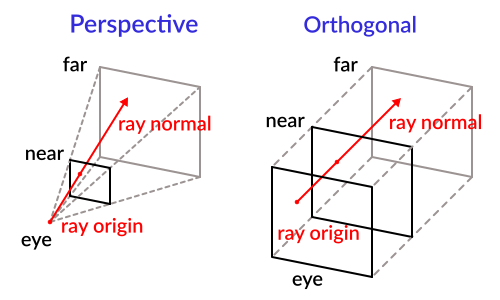
\includegraphics[width=.95\linewidth]{img/04/raycast_projection.png} 
        \caption{Deux types de projections}
 		\label{fig:raycast_projection}
\end{figure}


\subsection{la réduction de la ligne de visée}

Dans les cas l'objectif est de réduire une ligne de visée a une valeurs a représenter a l’écran.
Il existe plusieurs façons de réduire les lignes de visées.

Une des méthodes les plus facile consiste a prendre la moyenne ou la somme de la ligne, cette méthode présente l'avantage de représenter l'ensemble de la ligne.
Il est également possible de prendre les maximum de la ligne, cette méthode augmente significativement le contraste, au point que certaines projections peuvent présenter des artefacts indésirables.

Une troisième méthodes légèrement plus physique consiste a utiliser les équations de transfert du rayonnment pour determiner l'epaisseur optique de la ligne

\begin{equation}
v= \sum e^{-d}
\end{equation}

Enfin, il est possible d'utilisé la réelle expression de l'epaisseur optique, prenant en compte densité, température, ionization et vitesse du gaz.
(TODO)


\subsection{Projection orthogonale}
J'ai develloper une methode de projection d'AMR utilisant les fonction hystograme de numpy.
Ces fonctions étant tres optimisées, la performance de génération de cube est généralement satisfaisante (pour les cube L<10).
L'idée est de considéré les cellule AMR comme des particules d'une certaine taille.

Prenon l'exemple d'une grille de densité non raffiné utilisant les sorties EMMA.
Une grille 2d  quelconque est représenté par x,y,l et d ou x,y etant les position du bord inferieur guauche des cellules, l étant le niveau des cellules d etant le champs a représenter (ici la densité).

\begin{equation}
dV= \left( \frac{1}{2**L }\right) **3
\end{equation} 

En réalisant un histogram 2d de x et y pondéré en masse.
Le poids de chaque cellule correspond a la masse de la cellule $w = \rho \cdot dV$:
En considerant le centre des cellule $(x' = x+dx(L) /2)$ et en ajustant le bin de l'histograme sur la taille de la grille on peux projeter un niveau tres rapidement.

\begin{lstlisting}[float=bth,language=python,frame=tb,caption={lprojection de l'AMR par la méthode des histogramme Numpy},label=lst:useless]
 import numpy as np
 h,binX,binY=np.hystogram2d(x,y,weight=dv)
\end{lstlisting}

ou h est une matrice 2d representant la projection.


Lorsque l'AMR d'entrée contient plusieurs niveaux, il est possible de projeter les cellules niveau par niveau.
Par example pour une grille contenant les niveaux 8 et 9, on projettera d'abord toutes les cellules de niveau 8 pour obtenir une matrice 256x256.
puis on agrandira cette matrice avec des operateurs de changement de grille (TODO cf multigrille).
La méthode la plus naturelle consiste utiliser une projection directe.
nous obtenons alors une premiere grille de taille 512x512.
On projettera ensuite par histogramme toutes les cellules du niveau  9 pour obtenir une seconde matrice de taille 512x512.
La grille finale sera la moyenne des deux grille précédentes.

On pourra utiliser ce principe de manière récursive jusqu'a avoir projeter tout les niveaux.

Dans le cas ou le niveau de projection ne correspond pas au niveau maximum de l'AMR, il suffira de modifier la pondération des niveau superieur au niveau de projection en utilisant:

\begin{equation}
w = d \cdot \left( \frac{1}{2**(L-Lmax) }\right) **3
\end{equation}



L'inconveniant de la methode des histogramme est qu'il n'est possible de realiser que des projection utilisant la moyenne.
Or on voudra dans certain cas considérer d'autres reduction de ligne de visée.
Pour compenser cette methode on realisera une projection 3d de la même maniere que precedement mais en utilisant numpy.hystogramdd qui permet de realiser des histogrammes a N dimensions.
La taille de l'histogramme augmentant en 2**3L les projections 3d seront genéralement limité a 1024**3 pour des question de mémoire RAM. 





%matplotlib
%PIL
%openseadragon
%








\section{Projection perspective}
%opengl
%blender

Dans ce cas, il n'existe plus de façon directe de recuperer les lignes de visée, il est nécessaire d'avoir recours au lancé de rayon.
Cette technique appelée raycasting permet de récupérer toute les cellules interceptée pas un rayon donné.
Il existe différentes techniques de raycasting, j'ai pu en explorer plusieurs:

\subsection{L'algorithme de bressenham}
L'algorithme de bressenham est une technique optimisée de raycasting.
Il consiste a travailler sur l'indice des cellules d'une grille regulière.

Cette technique est tres rapide mais ne fonctionne cependant que sur grille regulière.

\begin{figure}[bth]
        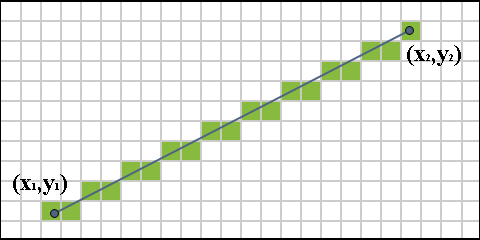
\includegraphics[width=.95\linewidth]{img/04/Bresenham_line.png} 
        \caption{Algorithme de Bressenham }
 		\label{fig:bressenham}
\end{figure}




\subsection{La méthodes KD-tree}

Une autre technique mise en place dans le but d'explorer directement l'amr.
De la mème manière que la technique de calcule des flux (TODO ref) cette technique repose sur l'utilisation d'un arbre pour determiner le cellule par lesquelles passent le rayon.





la mise en place de la camera
la définition de la position et du champs de vue (FOV) et de la profondeur de vue.
camera sphérique avec HealPix see Sec. \ref{sec:healpix}

la projection equirectangle est la projection la plus utilisée en photographie et video sphérique.
Elle présente un ratio d'aspect de 2:1 correspondant a 360:180.
L'association Healpix vers equirectangle est trivial puisque qu'elle consiste a associer les position x,y de la projection equirectangle, au angle $\theta$ et $\phi$ de la projection Healpix.
\begin{equation}
x=\theta
y=\phi
\end{equation}

La densité de point n'etant pas uniforme dans ce reférentiel, il est necessaire de realiser une interpolation sur une matrice régulière pour obtenir l'image finale. see Fig \ref{fig:equirectangle}


\begin{figure}[bth]
        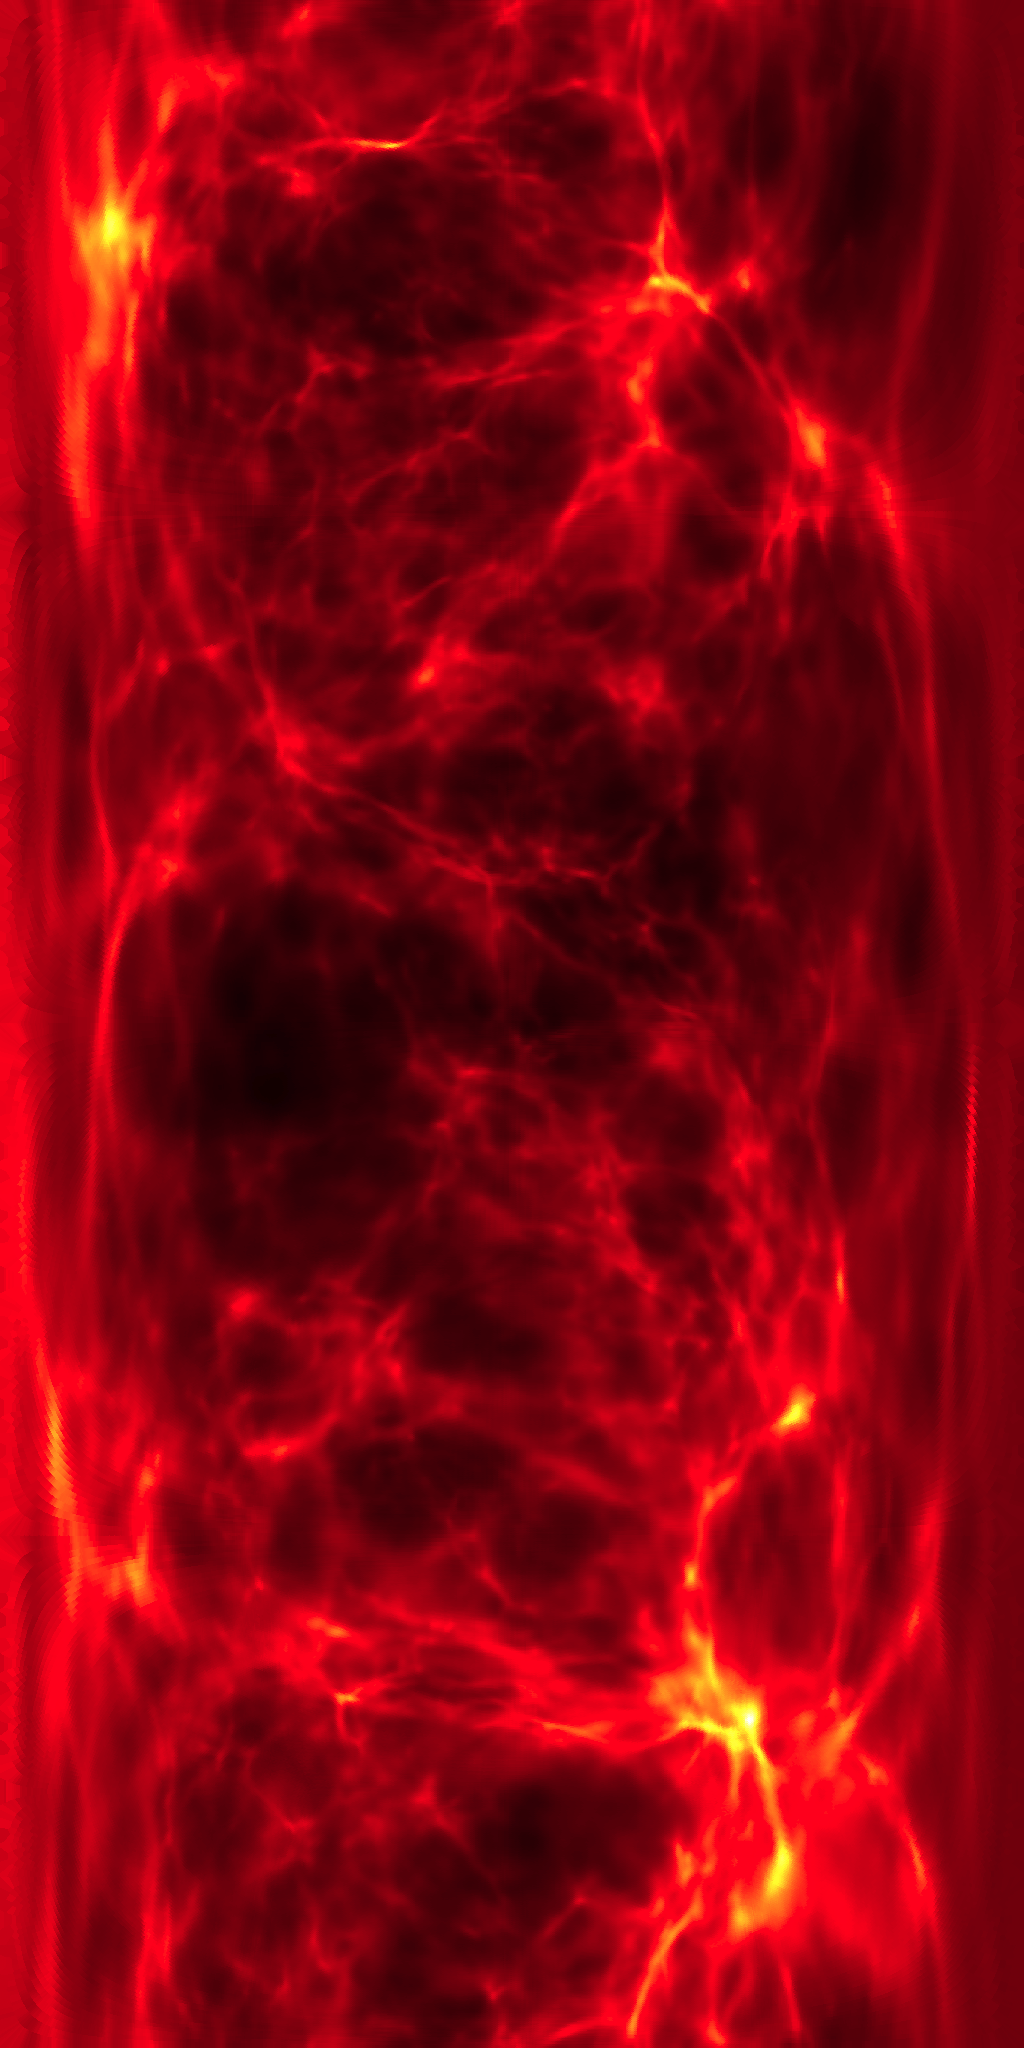
\includegraphics[height=.95\textheight]{img/04/equi.png} 
        \caption{Projection equirectangle d'une cube de densité}
 		\label{fig:equirectangle}
\end{figure}


\section{le compositing RGB (A)}
Une fois les projections realisées il est possibles de les combinées en créant des images en fausses couleurs.

De maniere naturelle, J'ai utilisé le rouge pour  la température et la transparence pour l'ionization.
il reste le bleu et le vert.
Dans une première série d'images j'ai utilisé le vert pour la densité de gas et le bleu pour la densité de matière noire.

\subsection{le théorie des couleurs}
Comment créer du noir et blanc?


par la moyenne :
\begin{equation}
gray= (R+G+B)/3
\end{equation}

R,G,B=gray


par une ponderation spéciale correspondant a la capacité de l'oeil a voir certaine couleur, conservation de la luminance:
\begin{equation}
gray = R*0.2989 + G*0.5870 +B*0.1140
\end{equation}

R,G,B=gray


\section{Movie}
implementation du mode movie de EMMA

c'est la même chose que précedemment mais a chaque pas de temps, il faut l'implementer en live (en c) pour ne pas avoir a sortir toute les info.

\section{Light cone}
A partir des images


\begin{figure}[bth]
        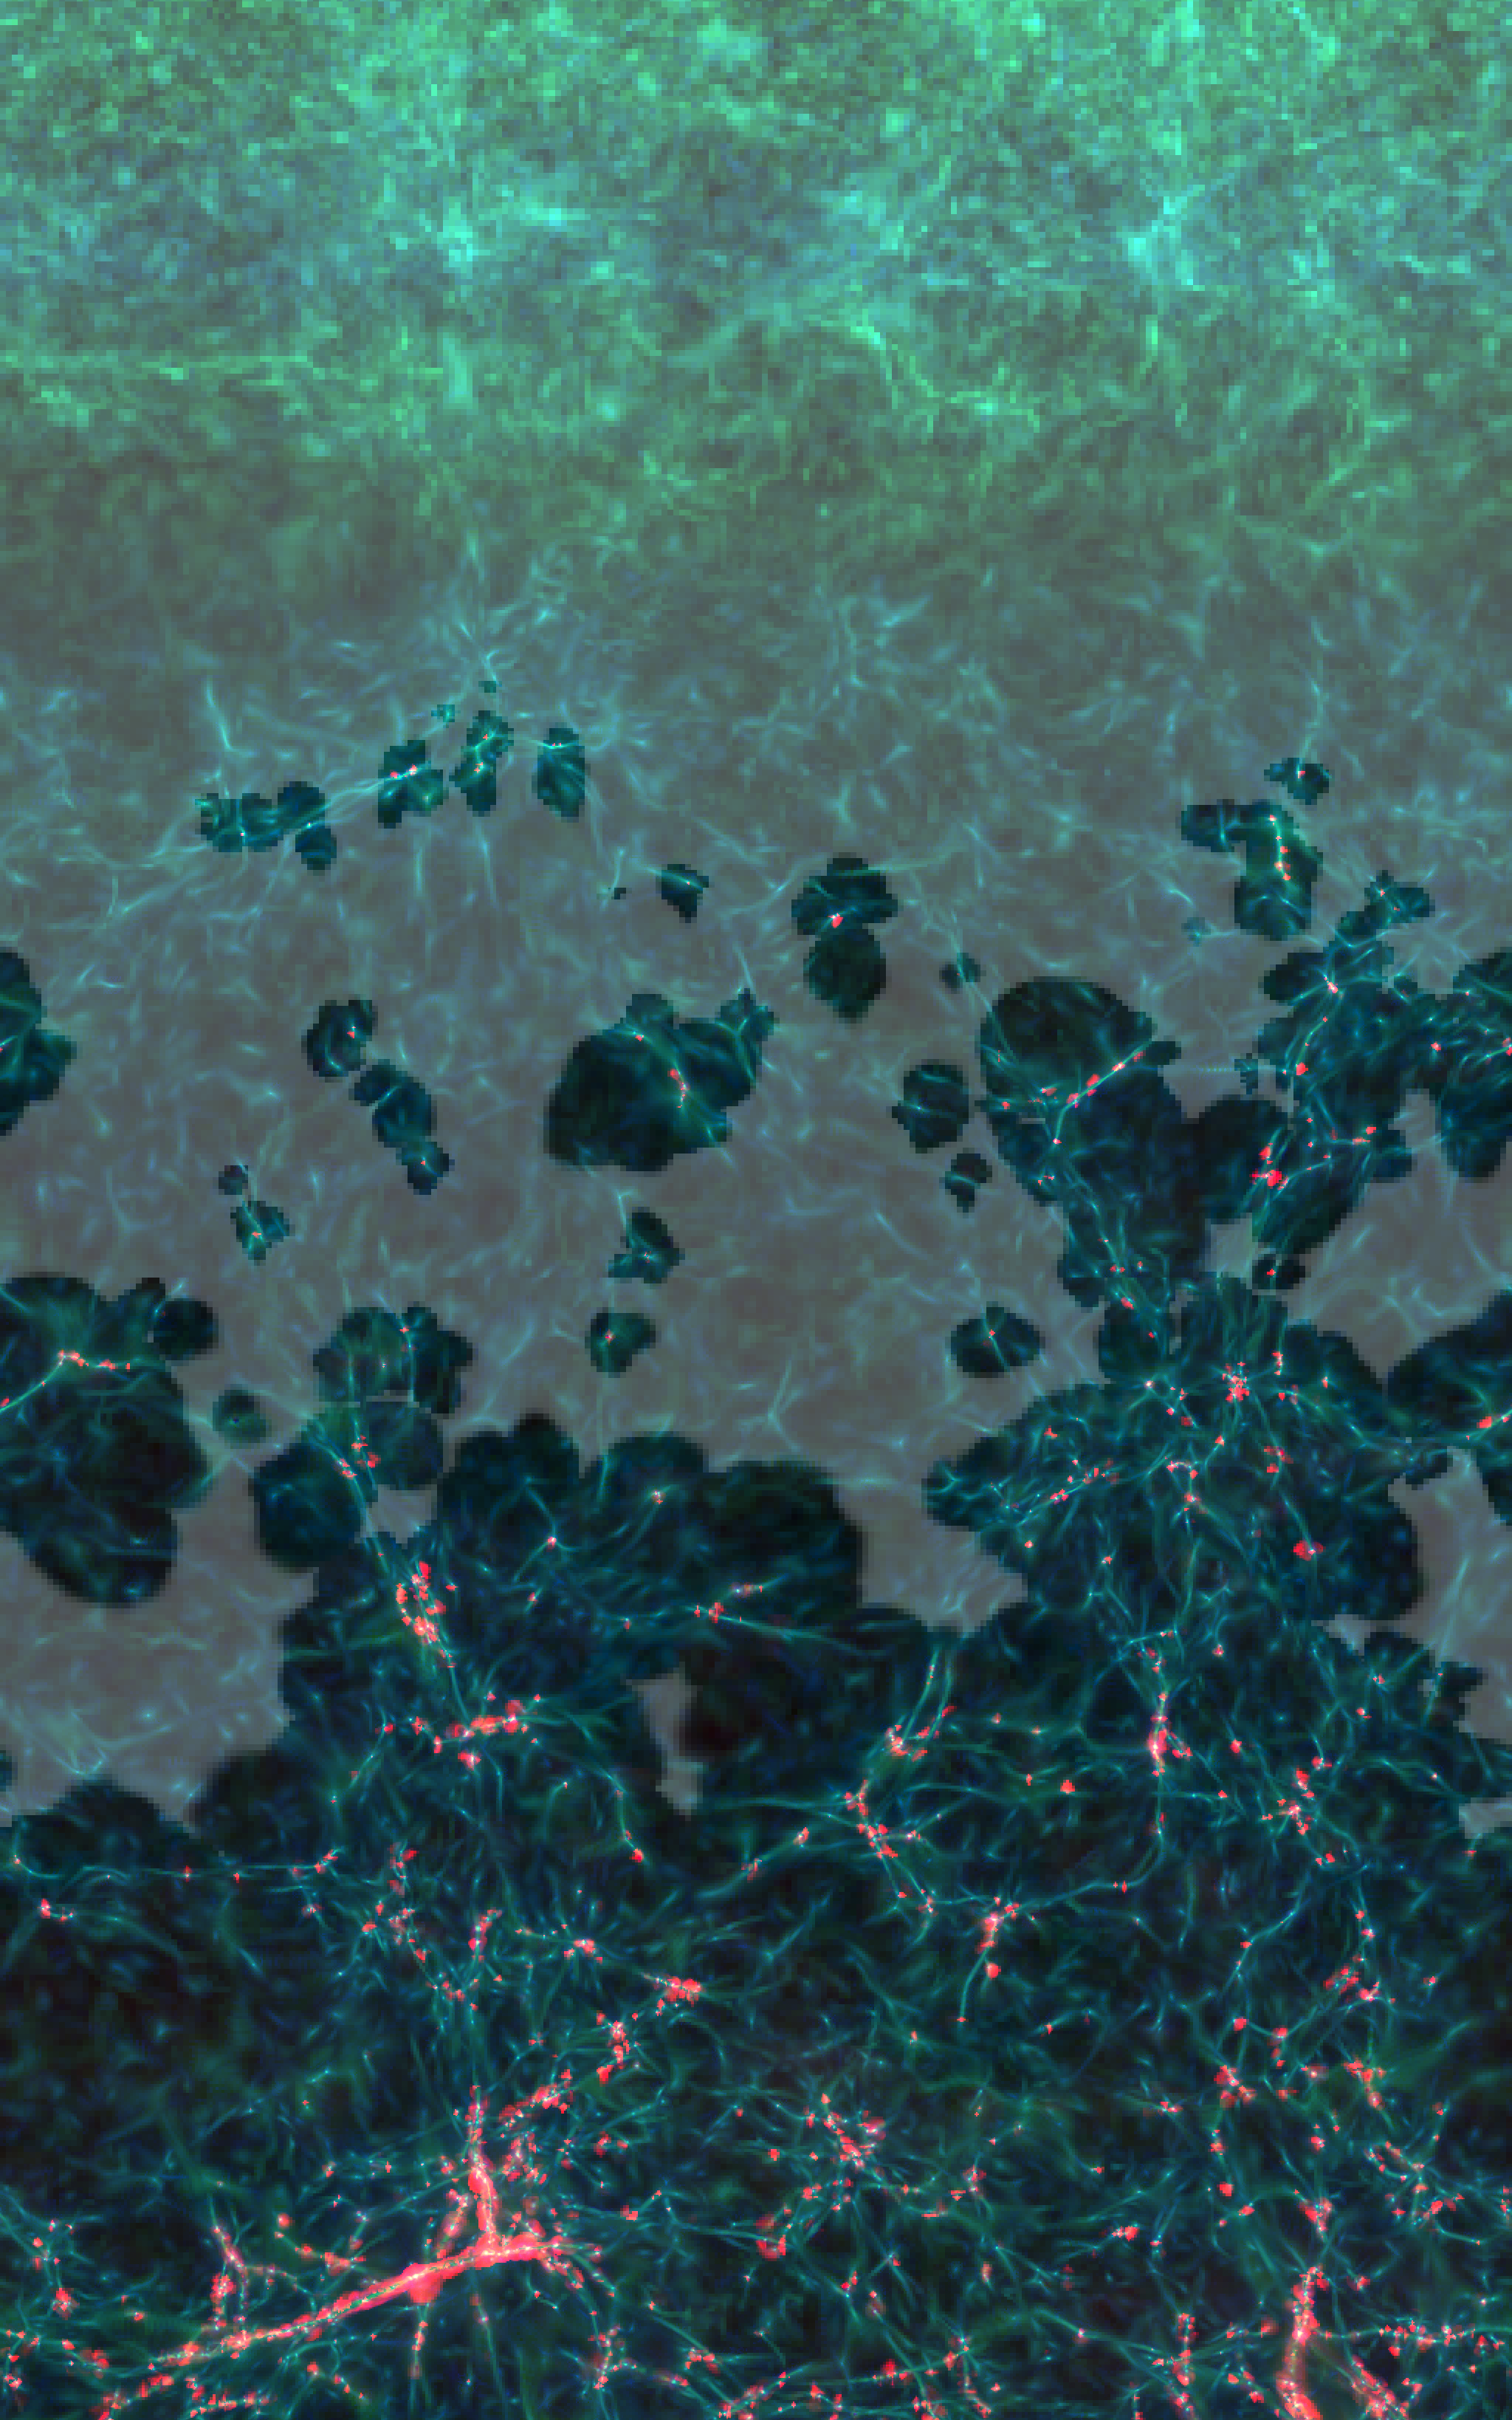
\includegraphics[height=.95\textheight]{img/04/frise_wall.png} 
        \caption{Light cone}
 		\label{fig:lightcone}
\end{figure}

